\nxsection{Les Alertes}\label{sec:administration-alertes}
\index{les alertes}

\nxsubsection{Afficher les d\'etails d'une alerte}
\index{afficher les d\'etails d'une alerte}

La figure~\ref{fig:admin-alertes-afficher-details} illustre
l'interface graphique de \yeroth qui affiche les d\'etails
d'une alerte.\\

\begin{figure}[!htpb]
	\centering
	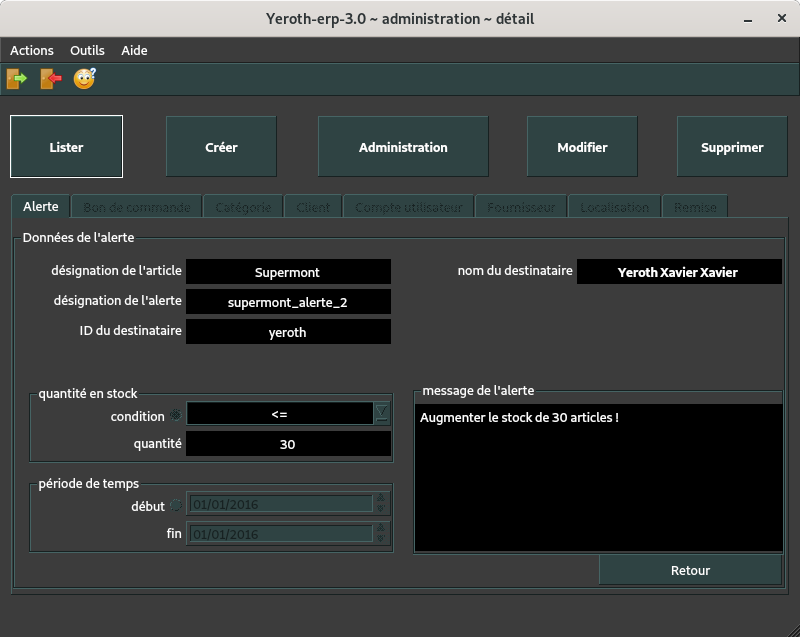
\includegraphics[scale=0.45]{images/alerte-afficher-details.png}
	\caption{Une interface graphique de \yeroth qui affiche les d\'etails
	d'une alerte.}\label{fig:admin-alertes-afficher-details}
\end{figure}

\procparagraph{Proc\'edure pour afficher les d\'etails d'une alerte}
\begin{enumerate}[1)]
	\item \`A partir de l'interface graphique de l'acceuil de
		l'administration (voir figure~\ref{fig:fenetre-administrateur}),
		on clique sur l'onglet intitul\'e \textbf{op\'erations}. 
		
	\item Choisir '\textbf{lister}' dans le '\emph{combo box
		op\'erations}'.
		
	\item Choisir '\textbf{une alerte}' dans le '\emph{combo box
		sujets}'. Vous \^etes automatiquement conduit \`a la fen\^etre
		illustr\'ee par la figure~\ref{fig:admin-alertes-lister}.
		
	\item S\'electionner l'alerte dont vous souhaitez afficher
		les d\'etails dans la liste des alertes affich\'ee.
		
	\item Cliquer sur le bouton \bouton{Afficher}. Les d\'etails
		sur le stock sont affich\'es dans une nouvelle fen\^etre.
\end{enumerate}

%%%%%%%%%%%%%%%%%%%%%%%%%%%%%%%%%%%%%%%%%%%%%%%%%%%%%%%%%%%%%%%%%%%%%%%%%%%%%%%%%

\newpage
\nxsubsection{Cr\'eer une alerte}\label{sec:administration-alertes-creer}
\index{cr\'eer une alerte}

La figure~\ref{fig:admin-alertes-creer} illustre l'interface
graphique de \yeroth pour cr\'eer une alerte.\\

\begin{figure}[!htpb]
	\centering
	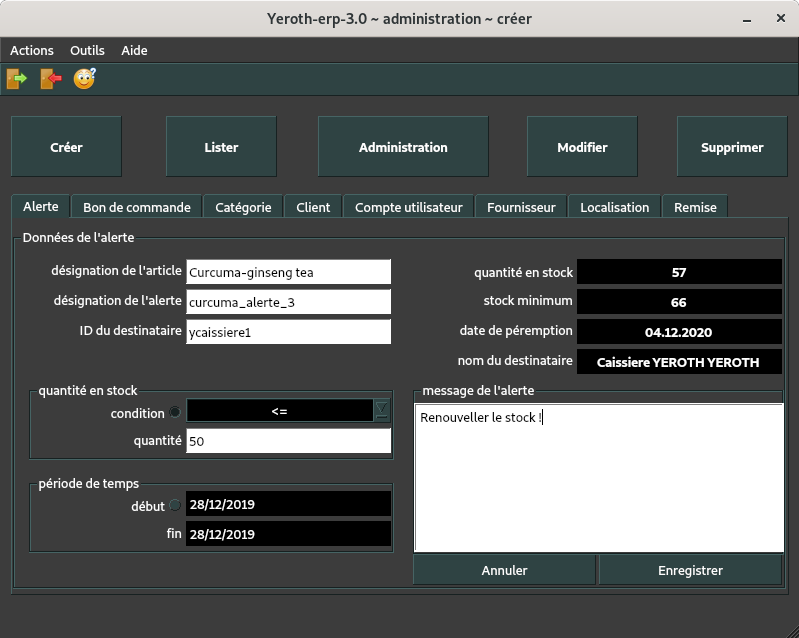
\includegraphics[scale=0.45]{images/alerte-creer.png}
	\caption{L'interface graphique pour cr\'eer des alertes.}
	\label{fig:admin-alertes-creer}
\end{figure}

\procparagraph{Proc\'edure pour cr\'eer une alerte}
Consulter les sections~\ref{sec:alerte-quantite-stock}
et~\ref{sec:alerte-periode-temps} pour savoir comment
cr\'eer respectivement des alertes sur la quantit\'e en
stock et des alertes sur la p\'eriode de temps.

%%%%%%%%%%%%%%%%%%%%%%%%%%%%%%%%%%%%%%%%%%%%%%%%%%%%%%%%%%%%%%%%%%%%%%%%%%%%%%%%%

\newpage
\nxsubsection{Lister les alertes}\label{sec:administration-alertes-lister}
\index{lister les alertes}

La figure~\ref{fig:admin-alertes-lister} illustre l'interface
graphique de \yeroth qui liste les alertes.\\

\begin{figure}[!htpb]
	\centering
	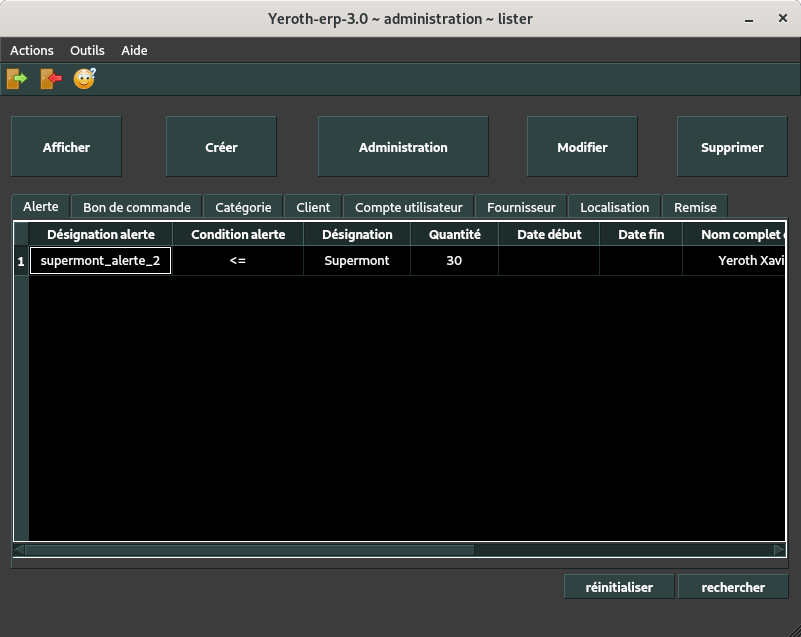
\includegraphics[scale=0.45]{images/alerte-lister.png}
	\caption{L'interface graphique qui liste les alertes.}
	\label{fig:admin-alertes-lister}
\end{figure}

\procparagraph{Proc\'edure pour lister les alertes}
\begin{enumerate}[1)]
	\item \`A partir de l'interface graphique de l'acceuil de
		l'administration (voir la figure~\ref{fig:fenetre-administrateur}),
		on clique sur l'onglet intitul\'e \textbf{op\'erations}. 
		
	\item Choisir '\textbf{lister}' dans le '\emph{combo box
		op\'erations}'.
		
	\item Choisir '\textbf{une alerte}' dans le '\emph{combo box
		sujets}'. Vous \^etes automatiquement conduit \`a la fen\^etre
		qui liste les alertes (voir la figure~\ref{fig:admin-alertes-lister}).
\end{enumerate}

%%%%%%%%%%%%%%%%%%%%%%%%%%%%%%%%%%%%%%%%%%%%%%%%%%%%%%%%%%%%%%%%%%%%%%%%%%%%%%%%%

\newpage
\nxsubsection{Modifier les d\'etails d'une alerte}
\index{modifier les d\'etails d'une alerte}

La figure~\ref{fig:admin-alertes-modifier} illustre
l'interface graphique de \yeroth pour modifier les
d\'etails d'une alerte.\\

\begin{figure}[!htpb]
	\centering
	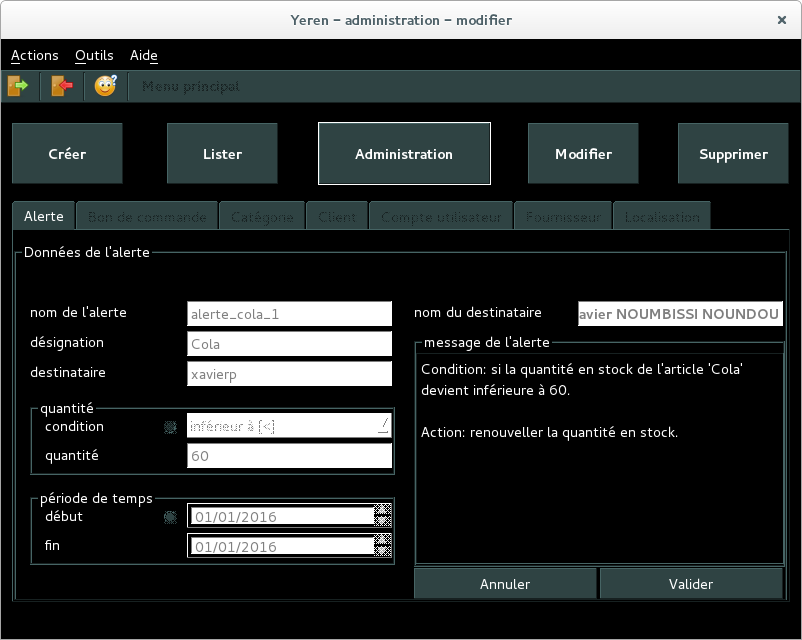
\includegraphics[scale=0.45]{images/alerte-modifier.png}
	\caption{L'interface graphique pour modifier les d'\'etails
	d'une alerte.}\label{fig:admin-alertes-modifier}
\end{figure}

\procparagraph{Proc\'edure pour modifier les d\'etails d'une alerte}
\begin{enumerate}[1)]
	\item \`A partir de l'interface graphique de l'acceuil de
		l'administration (voir figure~\ref{fig:fenetre-administrateur}),
		on clique sur l'onglet intitul\'e \textbf{op\'erations}. 
		
	\item Choisir '\textbf{lister}' dans le '\emph{combo box
		op\'erations}'.
		
	\item Choisir '\textbf{une alerte}' dans le '\emph{combo box
		sujets}'. Vous \^etes automatiquement conduit \`a la fen\^etre
		illustr\'ee par la figure~\ref{fig:admin-alertes-lister}.
		
	\item S\'electionner l'alerte dont vous souhaitez modifier
		les d\'etails dans la liste des alertes affich\'ee.
		
	\item Cliquer sur le bouton \bouton{Modifier}. Les d\'etails
		sur le stock sont affich\'es dans une nouvelle fen\^etre.
		
	\item Faites les modifications que vous souhaitez. Pour
		les alertes, seul le message d'alerte peut \^etre
		modifi\'e.
		
	\item Cliquer sur le bouton \bouton{valider} pour valider
		les modifications faites.
\end{enumerate}

%%%%%%%%%%%%%%%%%%%%%%%%%%%%%%%%%%%%%%%%%%%%%%%%%%%%%%%%%%%%%%%%%%%%%%%%%%%%%%%%%

\newpage
\nxsubsection{Supprimer une alerte}
\index{supprimer une alerte}

La figure~\ref{fig:admin-alertes-supprimer} illustre l'interface
graphique de \yeroth pour supprimer une alerte.\\

\begin{figure}[!htpb]
	\centering
	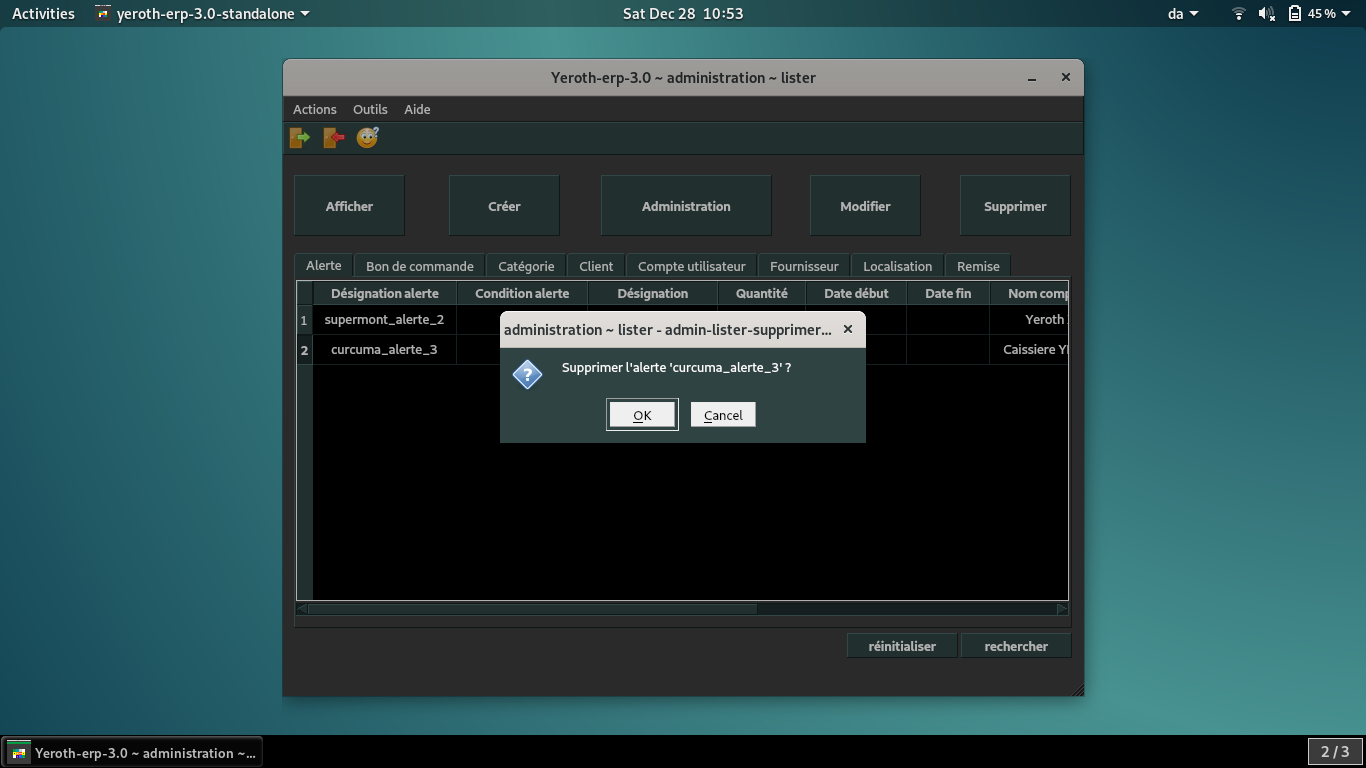
\includegraphics[scale=0.35]{images/alerte-supprimer.png}
	\caption{L'interface graphique pour supprimer des alertes.}
	\label{fig:admin-alertes-supprimer}
\end{figure}

\procparagraph{Proc\'edure pour supprimer une alerte}
\begin{enumerate}[1)]
	\item \`A partir de l'interface graphique de l'acceuil de
		l'administration (voir figure~\ref{fig:fenetre-administrateur}),
		on clique sur l'onglet intitul\'e \textbf{op\'erations}. 
		
	\item Choisir '\textbf{supprimer}' dans le '\emph{combo box
		op\'erations}'.
		
	\item Choisir '\textbf{une alerte}' dans le '\emph{combo box
		sujets}'. Vous \^etes automatiquement conduit \`a la fen\^etre
		illustr\'ee par la figure~\ref{fig:admin-alertes-lister}.
		
	\item S\'electionner l'alerte \`a supprimer dans la liste
		des alertes affich\'ee.
		
	\item Cliquer sur le bouton \bouton{Supprimer}. La question
		est ensuite pos\'ee si vous confirmer votre choix.
		Cliquer sur le \bouton{OK} pour confirmer votre choix.
\end{enumerate}
